% ====================================
\chapter{Les tableaux à 2 dimensions}
% ====================================

% ===================
\section{Définition}
% ===================

	\marginicon{definition}
	La \textbf{dimension} d’un tableau est le nombre d’indices qu’on utilise
	pour faire référence à un de ses éléments. Attention de ne pas confondre 
	avec la	taille !
	
	Dans ce qui précède, nous avons introduit les tableaux à une dimension.
	Un seul indice suffisait à localiser un de ses éléments. De nombreuses
	situations nécessitent cependant l’usage de tableaux à deux dimensions.
	Ils vous sont déjà familiers par leur présence dans beaucoup de
	situations courantes : calendrier, grille horaire, grille de mots
	croisés, sudoku, jeux se déroulant sur un quadrillage (damier,
	échiquier, scrabble \dots).

% ====================
\section{Déclaration}
% ====================

	\marginicon{definition}
	Pour déclarer un tableau statique à 2 dimensions, on écrira :

	\begin{Pseudocode}
	\Decl nomTableau : \K{tableau} [ligMin à ligMax, colMin à colMax] de TypeElément
	\end{Pseudocode}
	
	Pour un tableau dynamique, on procédera en deux étapes comme expliqué
	pour les tableaux à une dimension. 
	
	\begin{Pseudocode}
	\Decl nomTableau~: \K{tableau} de TypeElément
	\LComment Le code peut déterminer ici les bornes
	\Let nomTableau \Gets \K{nouveau} \K{tableau} [ligneMin à ligneMax, colMin à colMax] de TypeElément
	\end{Pseudocode}

	où \pseudocode{ligneMin}, \pseudocode{ligneMax}, 
	\pseudocode{colMin} et \pseudocode{colMax} sont des
	expressions entières quelconques.

	On ne se permettra pas en logique de
	combiner les deux types de tableaux, à savoir utiliser la notation
	«~statique~» pour certaines dimensions et «~dynamique~» pour les
	autres.

	Notez qu'un tableau à deux dimensions peut aussi être
	vu comme un tableau à une dimension dont chacun des éléments est
	lui-même un tableau à une dimension.

	\textbf{Exemple} : Soit le tableau déclaré ainsi:

	\begin{Pseudocode}
	\Decl ntabLettres : \K{tableau}[1 à 4, 1 à 5] de caractères
	\end{Pseudocode}

	On peut le visualiser à l’aide d’une grille à 4 lignes et 5 colonnes.

	\begin{center}
	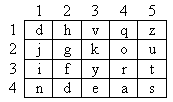
\includegraphics[width=4cm]{image/tab2d-vision-tab2d}
	\end{center}

	Ainsi, la valeur de \pseudocode{tabLettres[3,4]} 
	est le caractère ‘r’. 
	
	La vision «~tableau de tableau~» 
	(ou décomposition en niveaux)
	donnerait :

	\begin{center}
	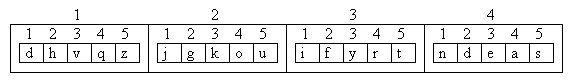
\includegraphics[width=0.9\textwidth]{image/tab2d-vision-tabtab}
	\end{center}

	Dans cette représentation, le tableau \pseudocode{tabLettres} est
	d’abord décomposé à un premier niveau en quatre éléments auxquels on
	accède par le premier indice. Ensuite, chaque élément de premier niveau
	est décomposé en cinq éléments de deuxième niveau accessibles par le
	deuxième indice.
	
	\textbf{Exemple~:} reprenons l'exemple du stock de 10 produits
	qui a servi d'introduction au chapitre sur les tableaux
	mais, cette fois, pour chaque jour de la semaine.
	
	\begin{small}
	\begin{center}
		\begin{tabular}{*{8}{>{\centering\arraybackslash}m{1.5cm}}}
			~ &
			{article1} &
			{article2} &
			{article3} &
			\dots &
			{article8} &
			{article9} &
			{article10}\\
		\end{tabular}	
		\begin{tabular}{|m{1.5cm}|*{7}{>{\centering\arraybackslash}m{1.5cm}|}}
			\hline
			{lundi} & 
			{cpt[1,1]} &
			{cpt[1,2]} &
			{cpt[1,3]} &
			\dots &
			{cpt[1,8]} &
			{cpt[1,9]} &
			{cpt[1,10]}
			\\\hline
			{mardi} &  
			{cpt[2,1]} &
			{cpt[2,2]} &
			{cpt[2,3]} &
			\dots &
			{cpt[2,8]} &
			{cpt[2,9]} &
			{cpt[2,10]}
			\\\hline
			{mercredi} & 
			{cpt[3,1]} &
			{cpt[3,2]} &
			{cpt[3,3]} &
			\dots &
			{cpt[3,8]} &
			{cpt[3,9]} &
			{cpt[3,10]}
			\\\hline
			{jeudi} & 
			{cpt[4,1]} &
			{cpt[4,2]} &
			{cpt[4,3]} &
			\dots &
			{cpt[4,8]} &
			{cpt[4,9]} &
			{cpt[4,10]}
			\\\hline
			{vendredi} & 
			{cpt[5,1]} &
			{cpt[5,2]} &
			{cpt[5,3]} &
			\dots &
			{cpt[5,8]} &
			{cpt[5,9]} &
			{cpt[5,10]}
			\\\hline
			{samedi} & 
			{cpt[6,1]} &
			{cpt[6,2]} &
			{cpt[6,3]} &
			\dots &
			{cpt[6,8]} &
			{cpt[6,9]} &
			{cpt[6,10]}
			\\\hline
			{dimanche} & 
			{cpt[7,1]} &
			{cpt[7,2]} &
			{cpt[7,3]} &
			\dots &
			{cpt[7,8]} &
			{cpt[7,9]} &
			{cpt[7,10]}
			\\\hline
		\end{tabular}
	\end{center}
	\end{small}
	
	\bigskip

	\begin{Pseudocode}
	\LComment Calcule et affiche la quantité vendue de 10 produits
	\LComment pour chaque jour de la semaine (de 1~: lundi à 7~: dimanche).
	\Module{statistiquesVentesSemaine}{}{}
		\Empty
		\Decl cpt~: \K{tableau} [1 à 7, 1 à 10] d’entiers
		\Decl produit, jour~: entiers
		\Empty
		\Stmt initialiser(cpt)
		\Empty
		\LComment Pour chaque jour de la semaine
		\For{jour \K{de} 1 \K{à} 7}
			\Stmt traiterStock1Jour(cpt, jour)
			\For{produit \K{de} 1 \K{à} 10}
				\Write "quantité vendue de produit ", produit, " ce jour ", jour, "~: ", cpt[jour][i]
			\EndFor
		\EndFor	
	\EndModule
	\end{Pseudocode}

	\begin{Pseudocode}
	\LComment Ce module initialise le tableau d'entiers à 0
	\Module{initialiser}{entiers\InOut~: \K{tableau} [1 à 7, 1 à 10] d’entiers}{}
		\Decl i, j~: entiers
		\For{i \K{de} 1 \K{à} 7}
			\For{j \K{de} 1 \K{à} 10}
				\Let cpt[i,j] \Gets 0
			\EndFor
		\EndFor
	\EndModule
	\end{Pseudocode}

	\begin{Pseudocode}
	\LComment Ce module effectue le traitement du stock pour une journée.
	\Module{traiterStock1Jour}{cpt~\InOut: \K{tableau} [1 à 7, 1 à 10] d’entiers, jour~: entier}{}
		\Decl numéroProduit, quantité~: entiers
		\Write "Introduisez le numéro du produit~:"
		\Read numéroProduit
		\Empty
		\While{numéroProduit > 0}
			\Empty
			\Write "Introduisez la quantité vendue~:"
			\Read quantité
			\Empty
			\Let cpt[jour,numéroProduit] \Gets cpt[jour,numéroProduit] + quantité
			\Empty
			\Write "Introduisez le numéro du produit~:"
			\Read numéroProduit
			\Empty
		\EndWhile
	\EndModule
	\end{Pseudocode}
	
	Pour plus d'exemples, allez faire un tour à la section \vref{algo:Tab2D}.

% ============================================
\section{La troisième dimension (et au-delà)}
% ============================================

	Certaines situations complexes nécessitent l'usage de
	tableaux à 3 voire plus de dimensions.

	\marginicon{definition}
	Pour déclarer un tableau statique à $k$ dimensions, on écrira :

	\begin{Pseudocode}
	\Decl nomTableau : \K{tableau} [ bMin\_1 à bMax\_1, \dots, bMin\_k à bMax\_k] de TypeElément
	\end{Pseudocode}

	où chaque paire de bornes \pseudocode{bMin\_i}~et
	\pseudocode{bMax\_i} limite l’indice correspondant 
	à la $i^{ème}$	dimension du tableau.
	
	
% ================================================
\section{Parcours d'un tableau à deux dimensions}
\label{algo:Tab2D}
% ================================================

Comme nous l'avons fait pour les tableaux à  une dimension,
envisageons le parcours des tableaux à deux dimensions 
(n lignes et m colonnes).

Déclaration d'un tableau statique~:

\begin{Pseudocode}
	\Decl tab~: tableau [1 à n, 1 à m] de T
\end{Pseudocode}

Déclaration d'un tableau dynamique~:

	\begin{Pseudocode}
	\Decl tab~: \K{tableau} de T
	\Let tab \Gets \K{nouveau} \K{tableau} [1 à n, 1 à m] de T
	\end{Pseudocode}

Commençons par des cas plus simples 
où on ne parcourt qu'une seule des dimensions 
puis attaquons le cas général.

\subsection{Parcours d'une dimension}

On peut vouloir ne parcourir qu'une seule ligne du tableau.
Si on parcourt la ligne $l$, on visite les cases 
$(l,1)$, $(l,2)$, \dots, $(l,m)$.
L'indice de ligne est constant et c'est l'indice de colonne qui varie.

\begin{center}
$l$
\begin{tabular}{|*{5}{>{\centering\arraybackslash}m{0.3cm}|}}
\hline
\ & \ & \ & \ & \  \\
\hline
\cellcolor{gray!25}\ & \cellcolor{gray!25}\ & \cellcolor{gray!25}\ & \cellcolor{gray!25}\ & \cellcolor{gray!25}\  \\
\hline
\ & \ & \ & \ & \  \\
\hline
\end{tabular}
\end{center}

Ce qui donne l'algorithme :

\begin{Pseudocode}
	\LComment{Parcours de la ligne $l$ d'un tableau à deux dimensions}
	\For{c de 1 à m}
		\Stmt traiter tab[l,c]
	\EndFor
\end{Pseudocode}

Retenons~: pour parcourir une ligne, on utilise une boucle sur les colonnes. 

Symétriquement, on pourrait considérer le parcours de la colonne $c$
comme avec l'algorithme suivant.

\begin{Pseudocode}
	\LComment{Parcours de la colonne $c$ d'un tableau à deux dimensions}
	\For{l de 1 à n}
		\Stmt traiter tab[l,c]
	\EndFor
\end{Pseudocode}

Si le tableau est carré ($n=m$) on peut aussi envisager le parcours
des deux diagonales.

Pour la diagonale descendante, 
les éléments à visiter sont $(1,1)$, $(2,2)$, \dots, $(n,n)$.

\begin{center}
\begin{tabular}{|*{3}{>{\centering\arraybackslash}m{0.3cm}|}}
\hline
\cellcolor{gray!25}\ & \ & \ \\
\hline
\ & \cellcolor{gray!25}\ & \ \\
\hline
\ & \ & \cellcolor{gray!25}\ \\
\hline
\end{tabular}
\end{center}

Une seule boucle suffit 
comme le montre l'algorithme suivant.

\begin{Pseudocode}
	\LComment{Parcours de la diagonale descendante d'un tableau carré}
	\For{i de 1 à n}
		\Stmt traiter tab[i,i]
	\EndFor
\end{Pseudocode}

Pour la diagonale montante, 
on peut envisager deux solutions, 
avec deux indices ou un seul
en se basant sur le fait que $i+j=n+1 \Rightarrow j=n+1-i$.

\begin{Pseudocode}
	\LComment{Parcours de la diagonale montante d'un tableau carré - 2 indices}
	\Let j \Gets n
	\For{i de 1 à n}
		\Stmt traiter tab[i,j]
		\Let j \Gets j - 1
	\EndFor
\end{Pseudocode}

\begin{Pseudocode}
	\LComment{Parcours de la diagonale montante d'un tableau carré - 1 indice}
	\For{i de 1 à n}
		\Stmt traiter tab[i, n + 1 - i]
	\EndFor
\end{Pseudocode}


\subsection{Parcours des deux dimensions}

\subsubsection*{Parcours par lignes et par colonnes}

Les deux parcours les plus courants sont les parcours ligne par ligne
et colonne par colonne.
Les tableaux suivants montrent dans quel ordre chaque case est visitée dans ces deux parcours.

\begin{center}
\begin{minipage}{0.4\textwidth}
\begin{center}
Parcours ligne par ligne\\
\begin{tabular}{|*{5}{>{\centering\arraybackslash}m{0.35cm}|}}
\hline
1 & 2 & 3 & 4 & 5 \\
\hline
6 & 7 & 8 & 9 & 10 \\
\hline
11 & 12 & 13 & 14 & 15 \\
\hline
\end{tabular}
\end{center}
\end{minipage}
\qquad
\begin{minipage}{0.4\textwidth}
\begin{center}
Parcours colonne par colonne\\
\begin{tabular}{|*{5}{>{\centering\arraybackslash}m{0.35cm}|}}
\hline
1 & 4 & 7 & 10 & 13 \\
\hline
2 & 5 & 8 & 11 & 14 \\
\hline
3 & 6 & 9 & 12 & 15 \\
\hline
\end{tabular}
\end{center}
\end{minipage}
\end{center}

Le plus simple est d'utiliser deux boucles imbriquées 

\begin{Pseudocode}
	\LComment{Parcours d'un tableau à 2 dimensions, ligne par ligne}
	\For{lg de 1 à n}
		\For{col de 1 à m}
			\Stmt traiter tab[lg,col]
		\EndFor
	\EndFor
\end{Pseudocode}

\begin{Pseudocode}
	\LComment{Parcours d'un tableau à 2 dimensions, colonne par colonne}
	\For{col de 1 à m}
		\For{lg de 1 à n}
			\Stmt traiter tab[lg,col]
		\EndFor
	\EndFor
\end{Pseudocode}

Mais on peut obtenir le même résultat avec une seule boucle
si l'indice sert juste à compter le nombre de passages
et que les indices de lignes et de colonnes sont gérés manuellement.

L'algorithme suivant montre ce que ça donne
pour un parcours ligne par ligne.
La solution pour un parcours colonne par colonne est similaire
et laissée en exercice.

\begin{Pseudocode}
	\LComment{Parcours d'un tableau à 2 dimensions via une seule boucle}
	\Let lg \Gets 1
	\Let col \Gets 1
	\For{i de 1 à n*m}
		\Stmt traiter tab[lg,col]
		\Let col \Gets col + 1	\RComment Passer à la case suivante
		\If{col > m} \RComment On déborde sur la droite, passer à la ligne suivante
			\Let col \Gets 1
			\Let lg \Gets lg + 1
		\EndIf
	\EndFor
\end{Pseudocode}

L'avantage de cette solution apparaitra 
quand on verra des situations plus difficiles.

\subsubsection*{Interrompre le parcours}

Comme avec les tableaux à une dimension, 
envisageons l'arrêt prématuré lors de la rencontre d'une certaine condition.
Et, comme avec les tableaux à une dimension, 
transformons d'abord nos \K{pour} en \K{tant que}.

Par exemple, montrons les deux parcours ligne par ligne, avec une et deux boucle(s).

\begin{Pseudocode}
	\LComment{Parcours d'un tableau à 2 dimensions, ligne par ligne, via un tant que}
	\Let lg \Gets 1
	\While{lg $\le$ n}
		\Let col \Gets 1
		\While{col $\le$ m}
			\Stmt traiter tab[lg, col]
			\Let col \Gets col + 1
		\EndWhile
		\Let lg \Gets lg + 1
	\EndWhile
\end{Pseudocode}

\begin{Pseudocode}
	\LComment{Parcours d'un tableau à 2 dimensions via une seule boucle et un tant que}
	\Let lg \Gets 1
	\Let col \Gets 1
	\Let i \Gets 1
	\While{i $\le$ n*m} \RComment ou "lg $\le$ n" 
		\Stmt traiter tab[lg,col]
		\Let col \Gets col + 1	\RComment Passer à la case suivante
		\If{col > m} \RComment On déborde sur la droite, passer à la ligne suivante
			\Let col \Gets 1
			\Let lg \Gets lg + 1
		\EndIf
		\Let i \Gets i + 1		
	\EndWhile
\end{Pseudocode}

On peut à présent introduire le test comme on l'a fait 
dans les algorithmes de parcours des tableaux à une dimension.

Illustrons-le au travers de deux exemples.
Le premier introduit un test en utilisant un booléen
alors que le second introduit un test
sans utiliser de booléen.

\begin{Pseudocode}
	\LComment{Parcours avec test d'arrêt - deux boucles et un booléen}
	\Let trouvé \Gets faux
	\Let lg \Gets 1
	\While{lg $\le$ n ET NON trouvé}
		\Let col \Gets 1
		\While{col $\le$ m ET NON trouvé}
			\If{\textit{tab[lg, col] impose l'arrêt du parcours}}
				\Let trouvé \Gets vrai
			\Else \RComment Ne pas modifier les indices si arrêt demandé
				\Let col \Gets col + 1
			\EndIf
		\EndWhile
		\If{NON trouvé} \RComment Ne pas modifier les indices si arrêt demandé
			\Let lg \Gets lg + 1
		\EndIf
	\EndWhile
\end{Pseudocode}

\begin{Pseudocode}
	\LComment{Parcours avec test d'arrêt - une boucle et pas de booléen}
	\Let lg \Gets 1
	\Let col \Gets 1
	\Let i \Gets 1
	\While{i $\le$ n*m ET \textit{tab[lg, col] n'impose pas l'arrêt}}  
		\Let col \Gets col + 1	\RComment Passer à la case suivante
		\If{col > m} \RComment On déborde sur la droite, passer à la ligne suivante
			\Let col \Gets 1
			\Let lg \Gets lg + 1
		\EndIf
		\Let i \Gets i + 1		
	\EndWhile
	\LComment Arrêt prématuré si i $\le$ n*m.
\end{Pseudocode}

\subsubsection*{Parcours plus compliqué - le serpent}

Envisageons un parcours plus difficile illustré par le tableau suivant.

\begin{center}
\begin{tabular}{|*{5}{>{\centering\arraybackslash}m{0.35cm}|}}
\hline
1 & 2 & 3 & 4 & 5 \\
\hline
10 & 9 & 8 & 7 & 6 \\
\hline
11 & 12 & 13 & 14 & 15 \\
\hline
\end{tabular}
\end{center}

Le plus simple est d'adapter l'algorithme de parcours 
avec une seule boucle
en introduisant un sens de déplacement, 
ce qui donne l'algorithme :

\begin{Pseudocode}
	\LComment{Parcours du serpent dans un tableau à deux dimensions}
	\Let lg \Gets 1
	\Let col \Gets 1
	\Let depl \Gets 1	\RComment 1 pour avancer, -1 pour reculer
	\For{i de 1 à n*m}
		\Stmt traiter tab[lg, col]
		\If{1 $\le$ col + depl ET col + depl $\le$ m}
			\Let col \Gets col + depl \RComment On se déplace dans la ligne
		\Else
			\Let lg \Gets lg + 1	\RComment On passe à la ligne suivante
			\Let depl \Gets -depl	\RComment et on change de sens
		\EndIf
	\EndFor
\end{Pseudocode}

% ===================
\section{Exercices}
% ===================

\begin{Exercice}{Affichage}
	Écrire un module qui affiche tous les éléments d'un
	tableau à $n$ lignes et $m$ colonnes
	\begin{enumerate}[label=\alph*)]
	\item ligne par ligne ;
	\item colonne par colonne.
	\end{enumerate}
\end{Exercice}

\begin{Exercice}{Les nuls}
	\marginicon{java}
	Écrire un module qui reçoit un tableau ($n$ x $m$)
	d'entiers et qui affiche la proportion
	d'éléments nuls dans ce tableau.
\end{Exercice}

\begin{Exercice}{Le contour du tableau}
	\marginicon{java}
	On donne un tableau d’entiers \pseudocode{tabEnt} 
	à $n$ lignes et $m$ colonnes. 
	Écrire un module retournant la somme 
	de tous les éléments \textit{impairs}
	situés sur le bord du tableau.

	Exemple : pour le tableau suivant, le module doit renvoyer $32$

	\begin{center}
	\begin{tabular}{|*{4}{>{\centering\arraybackslash}m{0.6cm}|}}
	  \hline
	  3 & 4 & 6 & 11\\\hline
	  2 & 21 & 7 & 9\\\hline
	  1 & 5 & 12 & 3\\\hline
	\end{tabular}
	\end{center}

	Et pour le suivant, le module doit renvoyer $6$

	\begin{center}
	\begin{tabular}{|*{5}{>{\centering\arraybackslash}m{0.3cm}|}}
	\hline
	 4 & 1 & 2 & 8 & 5\\\hline
	\end{tabular}
	\end{center}
\end{Exercice}

\begin{Exercice}{À vos pinceaux !}
	On possède un tableau à $n$ lignes et $n$ colonnes dont les éléments de type
	Couleur valent NOIR ou BLANC. On suppose que le tableau est initialisé
	à ‘BLANC’ au départ. Écrire un module qui ‘noircit’ les cases de ce
	tableau comme le suggèrent les dessins suivants~(les exemples sont
	donnés pour un tableau 10 x 10 mais les algorithmes doivent fonctionner
	quelle que soit la taille du tableau).
	
	\begin{center}
	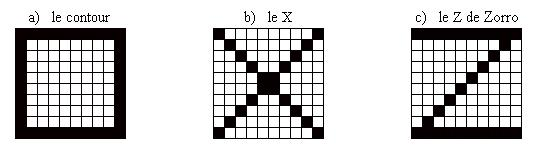
\includegraphics[width=0.9\textwidth]{image/tab2d-ex-oxz}
	\end{center}
\end{Exercice}

\begin{Exercice}{Le tableau de cotes}
	Soit un tableau à $n$ lignes et $m$ colonnes d'entiers où
	une ligne représente les notes sur 20 d'un étudiant et
	les colonnes toutes les notes d'un cours.
	
	Écrire un algorithme recevant ce tableau en paramètre et affichant le
	pourcentage d'étudiants ayant obtenu une moyenne
	supérieure à 50\%.
\end{Exercice}

\begin{Exercice}{Tous positifs}
	\marginicon{java}
	Écrire un module qui reçoit un tableau ($n$ x $m$) d’entiers et qui vérifie
	si tous les nombres qu’il contient sont strictement positifs. Bien sûr,
	on veillera à éviter tout travail inutile; la rencontre d’un nombre
	négatif doit arrêter le module.
\end{Exercice}

\begin{Exercice}{Le carré magique}
	\marginicon{java}
	Un carré magique est un tableau d’entiers carré
	(c'est-à-dire possédant autant de lignes que de
	colonnes) ayant la propriété suivante: si on additionne les éléments
	d'une quelconque de ses lignes, de ses colonnes ou de
	ses deux diagonales, on obtient à chaque fois le même résultat.

	Écrire un module recevant en paramètres le tableau [1 à $n$, 1 à $n$]
	d'entiers carré et renvoyant une valeur booléenne
	indiquant si Carré est un carré magique ou non.
\end{Exercice}

\begin{Exercice}{Le triangle de Pascal}
	Le triangle de Pascal est construit de la façon suivante :

	\begin{liste}
	\item la ligne initiale contient un seul élément de valeur 1 ;
	\item chaque ligne possède un élément de plus que la précédente ;
	\item chaque ligne commence et se termine par 1 ;
	\item 
		pour calculer un nombre d’une autre case du tableau, on additionne le
		nombre situé dans la case située juste au-dessus avec celui dans la
		case à la gauche de la précédente.
	\end{liste}

	Écrire un module qui reçoit en paramètre un entier
	$n$, et qui renvoie un tableau contenant les
	$n+1$ premières lignes du triangle de Pascal
	(indicées de $0$ à $n$).
	
	N.B.: le «~triangle~» sera bien entendu renvoyé dans un tableau carré.
	Quid des cases non occupées ?

	Par exemple, pour $n$ qui vaut 5, on aura le tableau suivant :

	\begin{center}
	\begin{tabular}{|*{6}{>{\centering\arraybackslash}m{0.35cm}|}}
	\hline
	 1 & ~ & ~ & ~ & ~ & ~ \\\hline
	 1 & 1 & ~ & ~ & ~ & ~ \\\hline
	 1 & 2 & 1 & ~ & ~ & ~ \\\hline
	 1 & 3 & 3 & 1 & ~ & ~ \\\hline
	 1 & 4 & 6 & 4 & 1 & ~ \\\hline
	 1 & 5 & 10 & 10 & 5 & 1 \\\hline
	\end{tabular}
	\end{center}
\end{Exercice}

\begin{Exercice}{Le calendrier du mois}
	Écrire un module qui reçoit en paramètres 
	le numéro du premier jour du mois 
	(c-à-d 1 si le mois commence un lundi, 2 si le mois commence un mardi,
	etc.) ainsi que le nombre de jours dans le mois.
	Au départ de ces données, 
	le module remplira avec les dates des jours du mois un tableau
	«~calendrier~» à deux dimensions, 
	dont les colonnes représentent les jours 
	(la première colonne correspondant au lundi) et les lignes les
	semaines. 
	Par exemple, si le mois contient 30 jours et le premier jour
	est un mercredi, le contenu du tableau sera :

	\begin{center}
	\begin{tabular}{|m{0.807cm}|m{0.807cm}|m{0.807cm}|m{0.807cm}|m{0.807cm}|m{0.807cm}|m{0.81100005cm}|}
	\multicolumn{1}{m{0.807cm}}{\centering 
	{L}} &
	\multicolumn{1}{m{0.807cm}}{\centering 
	{M}} &
	\multicolumn{1}{m{0.807cm}}{\centering 
	{M}} &
	\multicolumn{1}{m{0.807cm}}{\centering 
	{{J}}} &
	\multicolumn{1}{m{0.807cm}}{\centering 
	{{V}}} &
	\multicolumn{1}{m{0.807cm}}{\centering 
	{{S}}} &
	\multicolumn{1}{m{0.81100005cm}}{\centering\arraybslash
	 {D}}\\\hline
	~
	 &
	~
	 &
	\raggedleft  {1} &
	\raggedleft  {2} &
	\raggedleft  {3} &
	\raggedleft  {4} &
	\raggedleft\arraybslash 
	{5}\\\hline
	\raggedleft  {6} &
	\raggedleft  {7} &
	\raggedleft  {8} &
	\raggedleft  {9} &
	\raggedleft  {10} &
	\raggedleft  {11} &
	\raggedleft\arraybslash 
	{12}\\\hline
	\raggedleft  {13} &
	\raggedleft  {14} &
	\raggedleft  {15} &
	\raggedleft  {16} &
	\raggedleft  {17} &
	\raggedleft  {18} &
	\raggedleft\arraybslash 
	{19}\\\hline
	\raggedleft  {20} &
	\raggedleft  {21} &
	\raggedleft  {22} &
	\raggedleft  {23} &
	\raggedleft  {24} &
	\raggedleft  {25} &
	\raggedleft\arraybslash 
	{26}\\\hline
	\raggedleft  {27} &
	\raggedleft  {28} &
	\raggedleft  {29} &
	\raggedleft  {30} &
	~
	 &
	~
	 &
	~
	\\\hline
	\end{tabular}
	\end{center}

	\textbf{Réflexions} :

	\begin{liste}
	\item Combien de lignes au maximum doit avoir ce tableau ?
	\item Quid des cases non occupées ?
	\end{liste}
\end{Exercice}

\begin{Exercice}{À vos pinceaux (la suite) !}
	Pour poursuivre l'exercice du pinceau, 
	voici quelques cas plus coriaces.
	
	\begin{center}
	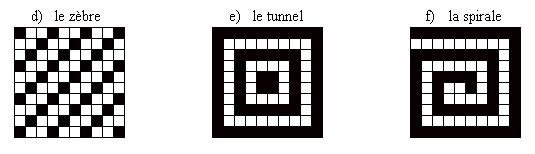
\includegraphics[width=0.9\textwidth]{image/tab2d-ex-zts}
	\end{center}
\end{Exercice}

\begin{Exercice}{Exercices sur la complexité}

	Quelle est la complexité 
	\begin{enumerate}[label=\alph*)]
	\item 
		d’un algorithme de parcours	d'un tableau $n$ x $n$ ?
	\item
		d'un algorithme qui remet à 0 toutes les
		occurrences du maximum d'un tableau $n$ x $n$ ?
	\item 
		de l'algorithme que vous avez écrit pour résoudre les
		exercices du pinceau ?
	\end{enumerate}
\end{Exercice}

\begin{Exercice}{Lignes et colonnes}
	Écrire un module qui reçoit un tableau d’entiers à 2 dimensions en paramètre 
	et qui retourne un booléen indiquant si ce tableau 
	possède 2 lignes ou 2 colonnes identiques.
	
	Dans l’affirmative, 
	ce module renverra également en paramètres les informations suivantes :
	
	\begin{liste}
	\item les indices des lignes ou colonnes identiques
	\item un caractère valant ‘L’ ou ‘C’ selon qu’il s’agit de lignes ou de
	colonnes
	\end{liste}
	
	Dans la négative, les valeurs de ces paramètres seront indéterminées ou
	quelconques, elles ne seront de toute façon pas utilisées par le module
	appelant.
\end{Exercice}
